\documentclass{article}

\usepackage{amsmath}
\usepackage{graphicx}

\addtolength{\oddsidemargin}{-.3in}
\addtolength{\evensidemargin}{-.3in}
\addtolength{\textwidth}{0.6in}

\begin{document}

\title{Homework 4\\
       Parallel Sort}
\author{Geoffrey Ulman\\
        CSI702}
\date{March 2010}
\maketitle

\section{Design}

\section{Challenges}

\section{MPI Commands}
Like all MPI programs, the commands \verb!MPI_Init!, \verb!MPI_Comm_size!, \verb!MPI_Comm_rank!, and \verb!MPI_Finalize! were used to initialize and get basic information about the MPI environment. Because binning was calculated on the host node, \verb!MPI_Bcast! was used to distribute the bin edges to the other nodes. Data was sent using \verb!MPI_Isend! and both \verb!MPI_Irecv! and \verb!MPI_Recv! were used for receving data. Synchronous receives were used to  Finally, completion of the communications in each iteration was checked with \verb!MPI_Waitall!.

\section{Performance Analysis}

\begin{figure}
\centering
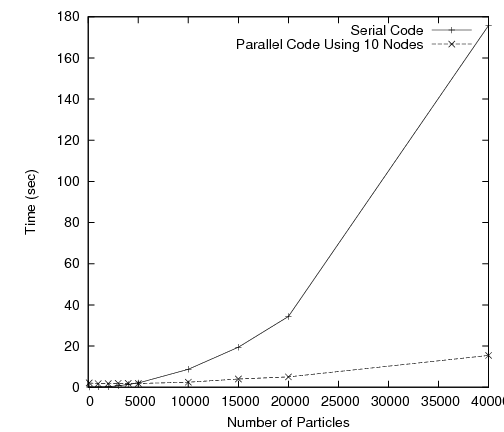
\includegraphics[width=0.6\textwidth]{img/timing_data_variable_particles.png}
\caption{Parallel and Serial Timing Results for Variable Particle Count}
\label{chart1}
\end{figure}


\section{Output Comparison}
\label{outputcomp}

\begin{thebibliography}{9}

\bibitem{cpl}
  Brian W. Kernighan and Dennis M. Ritchie,
  \emph{The C Programming Language},
  Prentice Hall PTR, New Jersey,
  2009.

\end{thebibliography}

\end{document}
